\section{Geometric Representation}
Consider the unit square and its diagonal. The length of this diagonal is precisely $\sqrt{2}$, giving us our first geometric insight into the number's nature. Each digit in the binary expansion can be thought of as a geometric construction:

\subsection{Diagram of Binary Expansion of \texorpdfstring{$\sqrt{2}$}{sqrt(2)}}

The diagram below illustrates several key concepts about the binary expansion of $\sqrt{2}$:
\begin{itemize}
    \item \textbf{Outer Square and Red Diagonal:} The black square represents 1 unit, and the red diagonal represents $\sqrt{2}$. Its infinite binary expansion is due to its irrationality.
    \item \textbf{Binary Approximation Process:} The nested blue dashed squares represent successive binary approximations, refining $\sqrt{2}$ to higher precision.
    \item \textbf{Green Circle:} This symbolizes the minimum "gap" that must exist between $\sqrt{2}$ and any rational approximation, ensuring no finite binary expansion can represent it exactly.
    \item \textbf{Zero Run Bounds:} Geometrically, runs of zeros correspond to maintaining a fixed level of approximation. These runs are bounded by $\log_2(n)$.
\end{itemize}

\begin{center}
    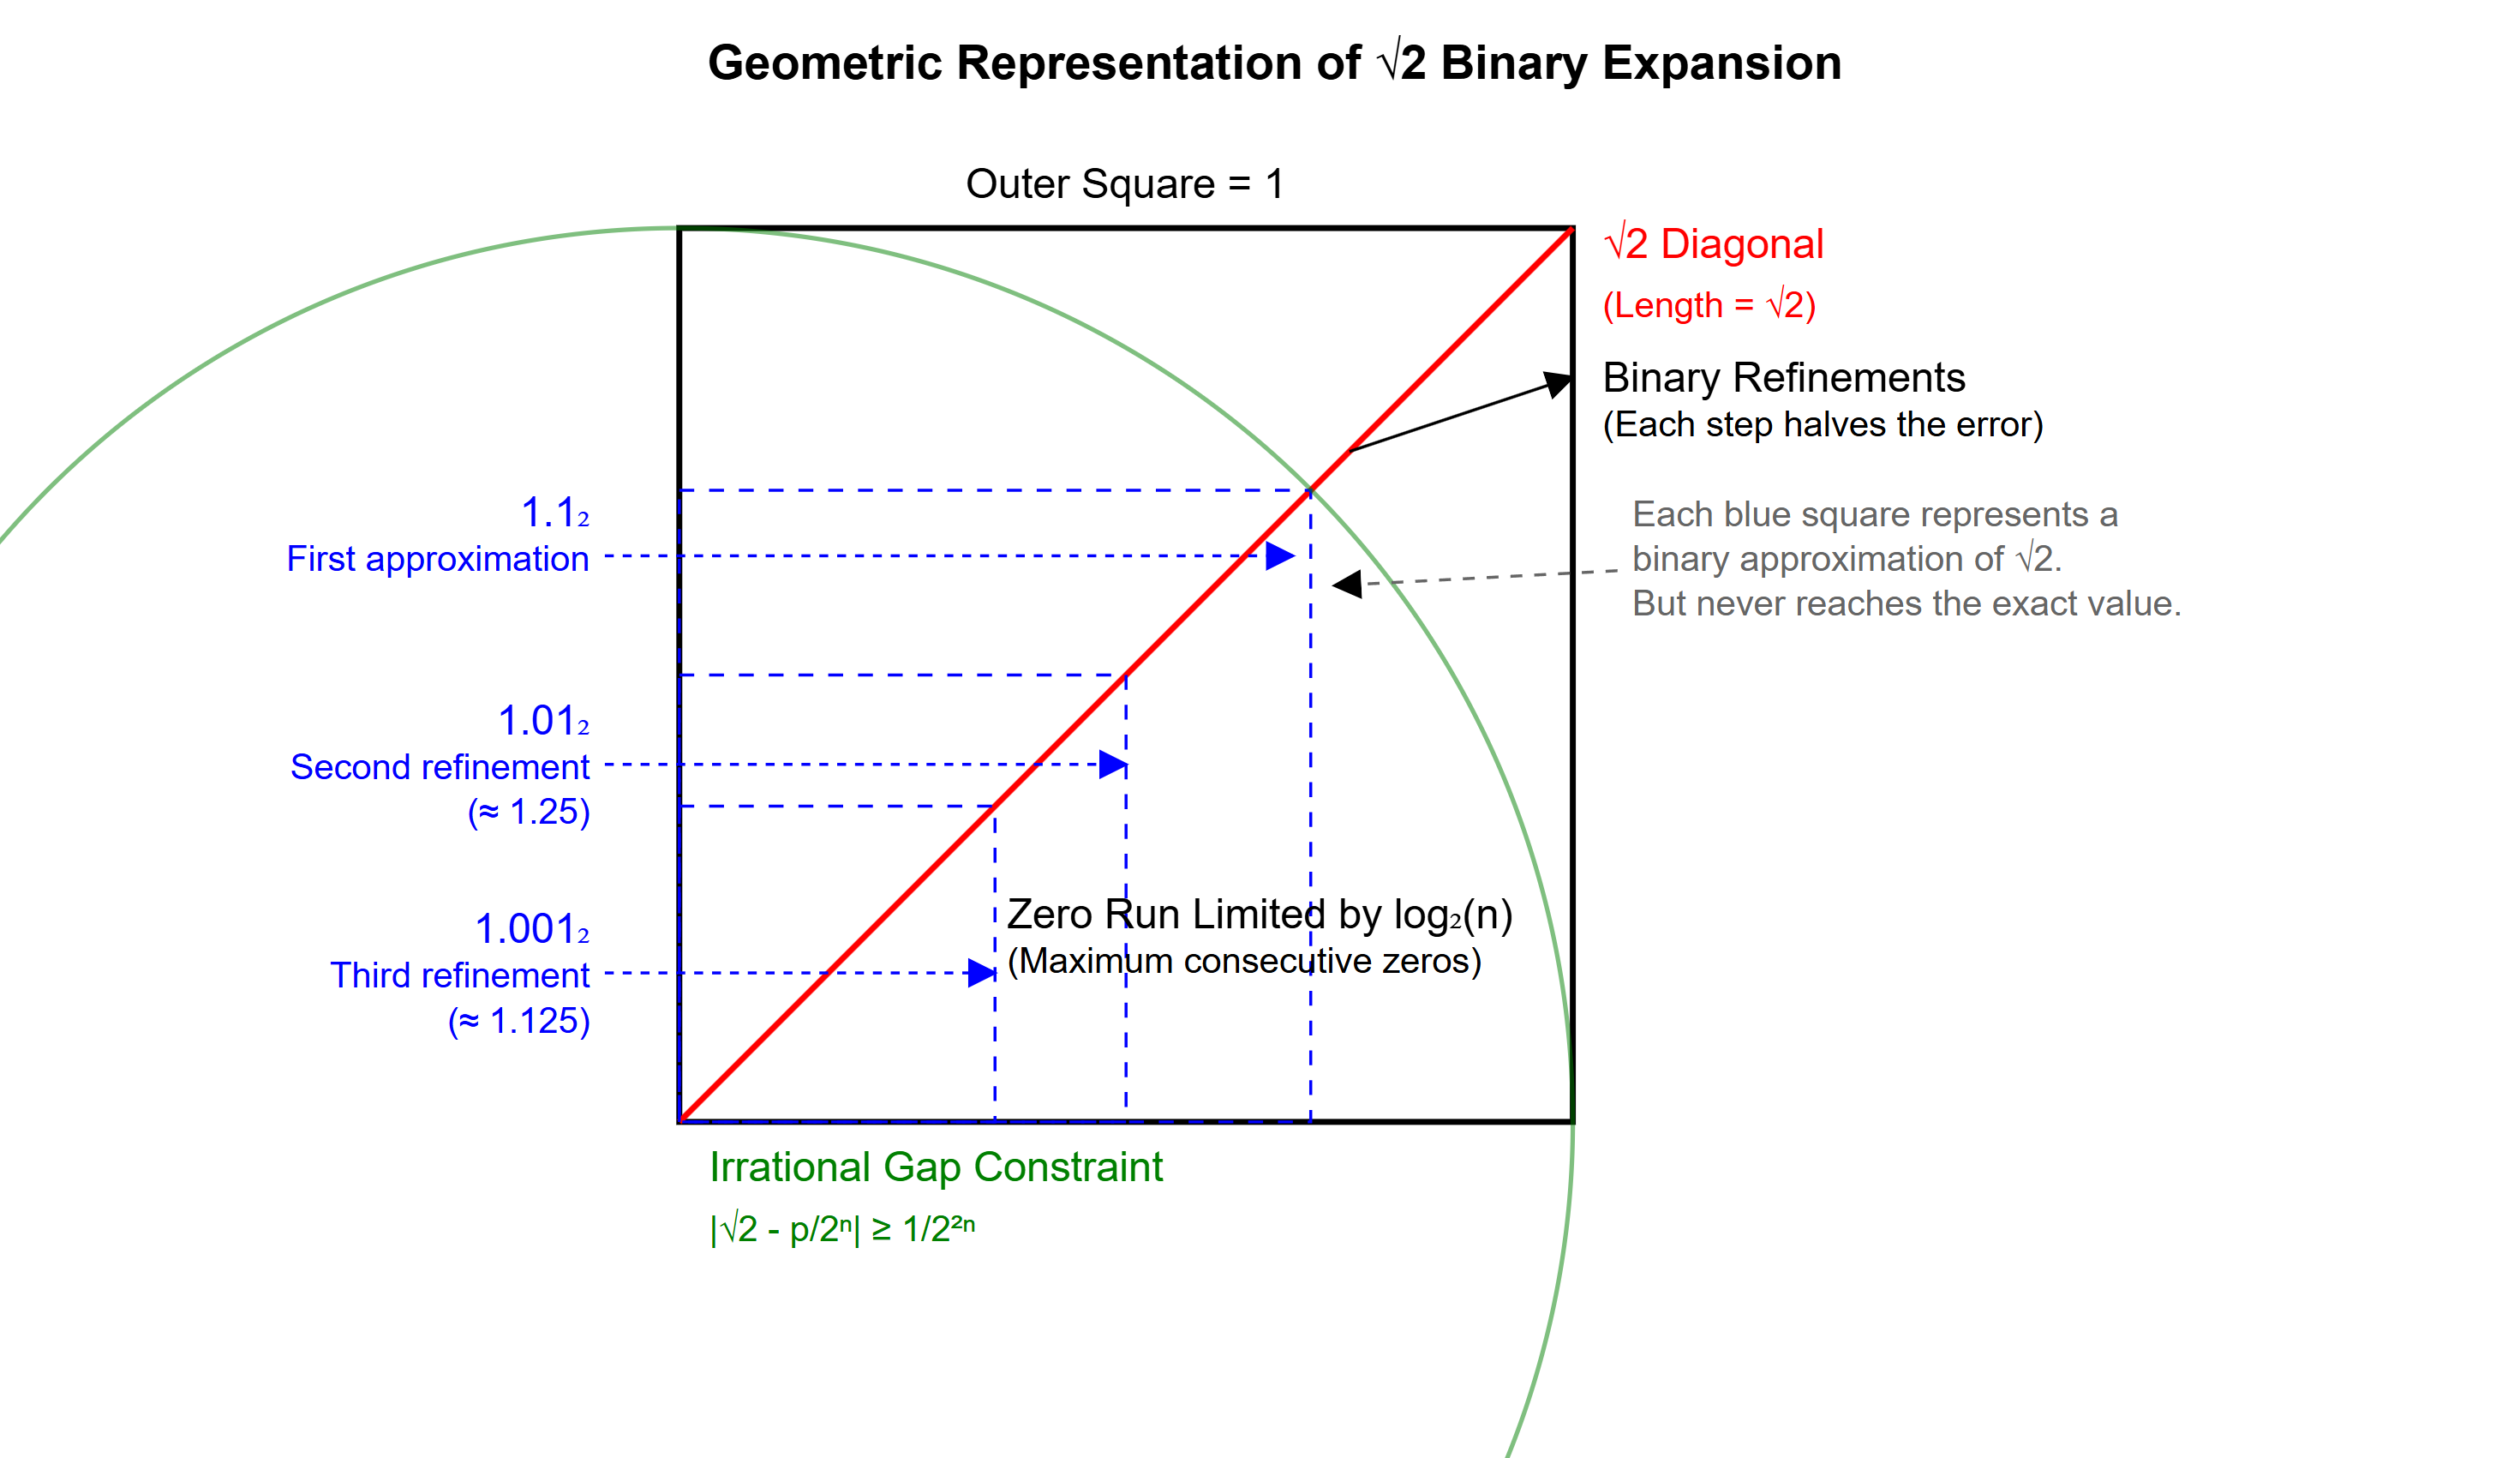
\includegraphics[width=0.8\textwidth]{geometric_diagram_illustrates.png} % Replace 'diagram.pdf' with your PDF file name
\end{center}


\subsection{Binary Expansion and Geometric Approximation}
Each binary digit represents a halving of the previous geometric step. A run of zeros in the binary expansion signifies a period where our approximation maintains its position relative to $\sqrt{2}$ without requiring adjustment. Geometrically, this translates to:

$$\sqrt{2} = 1.011010100000100111100\ldots_2$$

\subsection{The Geometric Constraint}
The key insight comes from understanding why runs of zeros must be limited. Consider a rational approximation $\frac{p}{2^n}$ of $\sqrt{2}$. Geometrically, this represents a point on our binary grid. For any such approximation:

$$\left|\sqrt{2} - \frac{p}{2^n}\right| \geq \frac{1}{2^{2n}}$$

This inequality has a beautiful geometric interpretation: it represents the minimum "gap" that must exist between any rational approximation and $\sqrt{2}$.

\subsection{Connection to Zero Runs}
A run of $k$ zeros in the binary expansion at position $n$ implies an approximation accurate to $2^{-k}$ at that position. The geometric constraint above tells us this accuracy cannot exceed certain bounds, directly leading to the $\log_2(n)$ limit on zero runs.

\begin{center}
    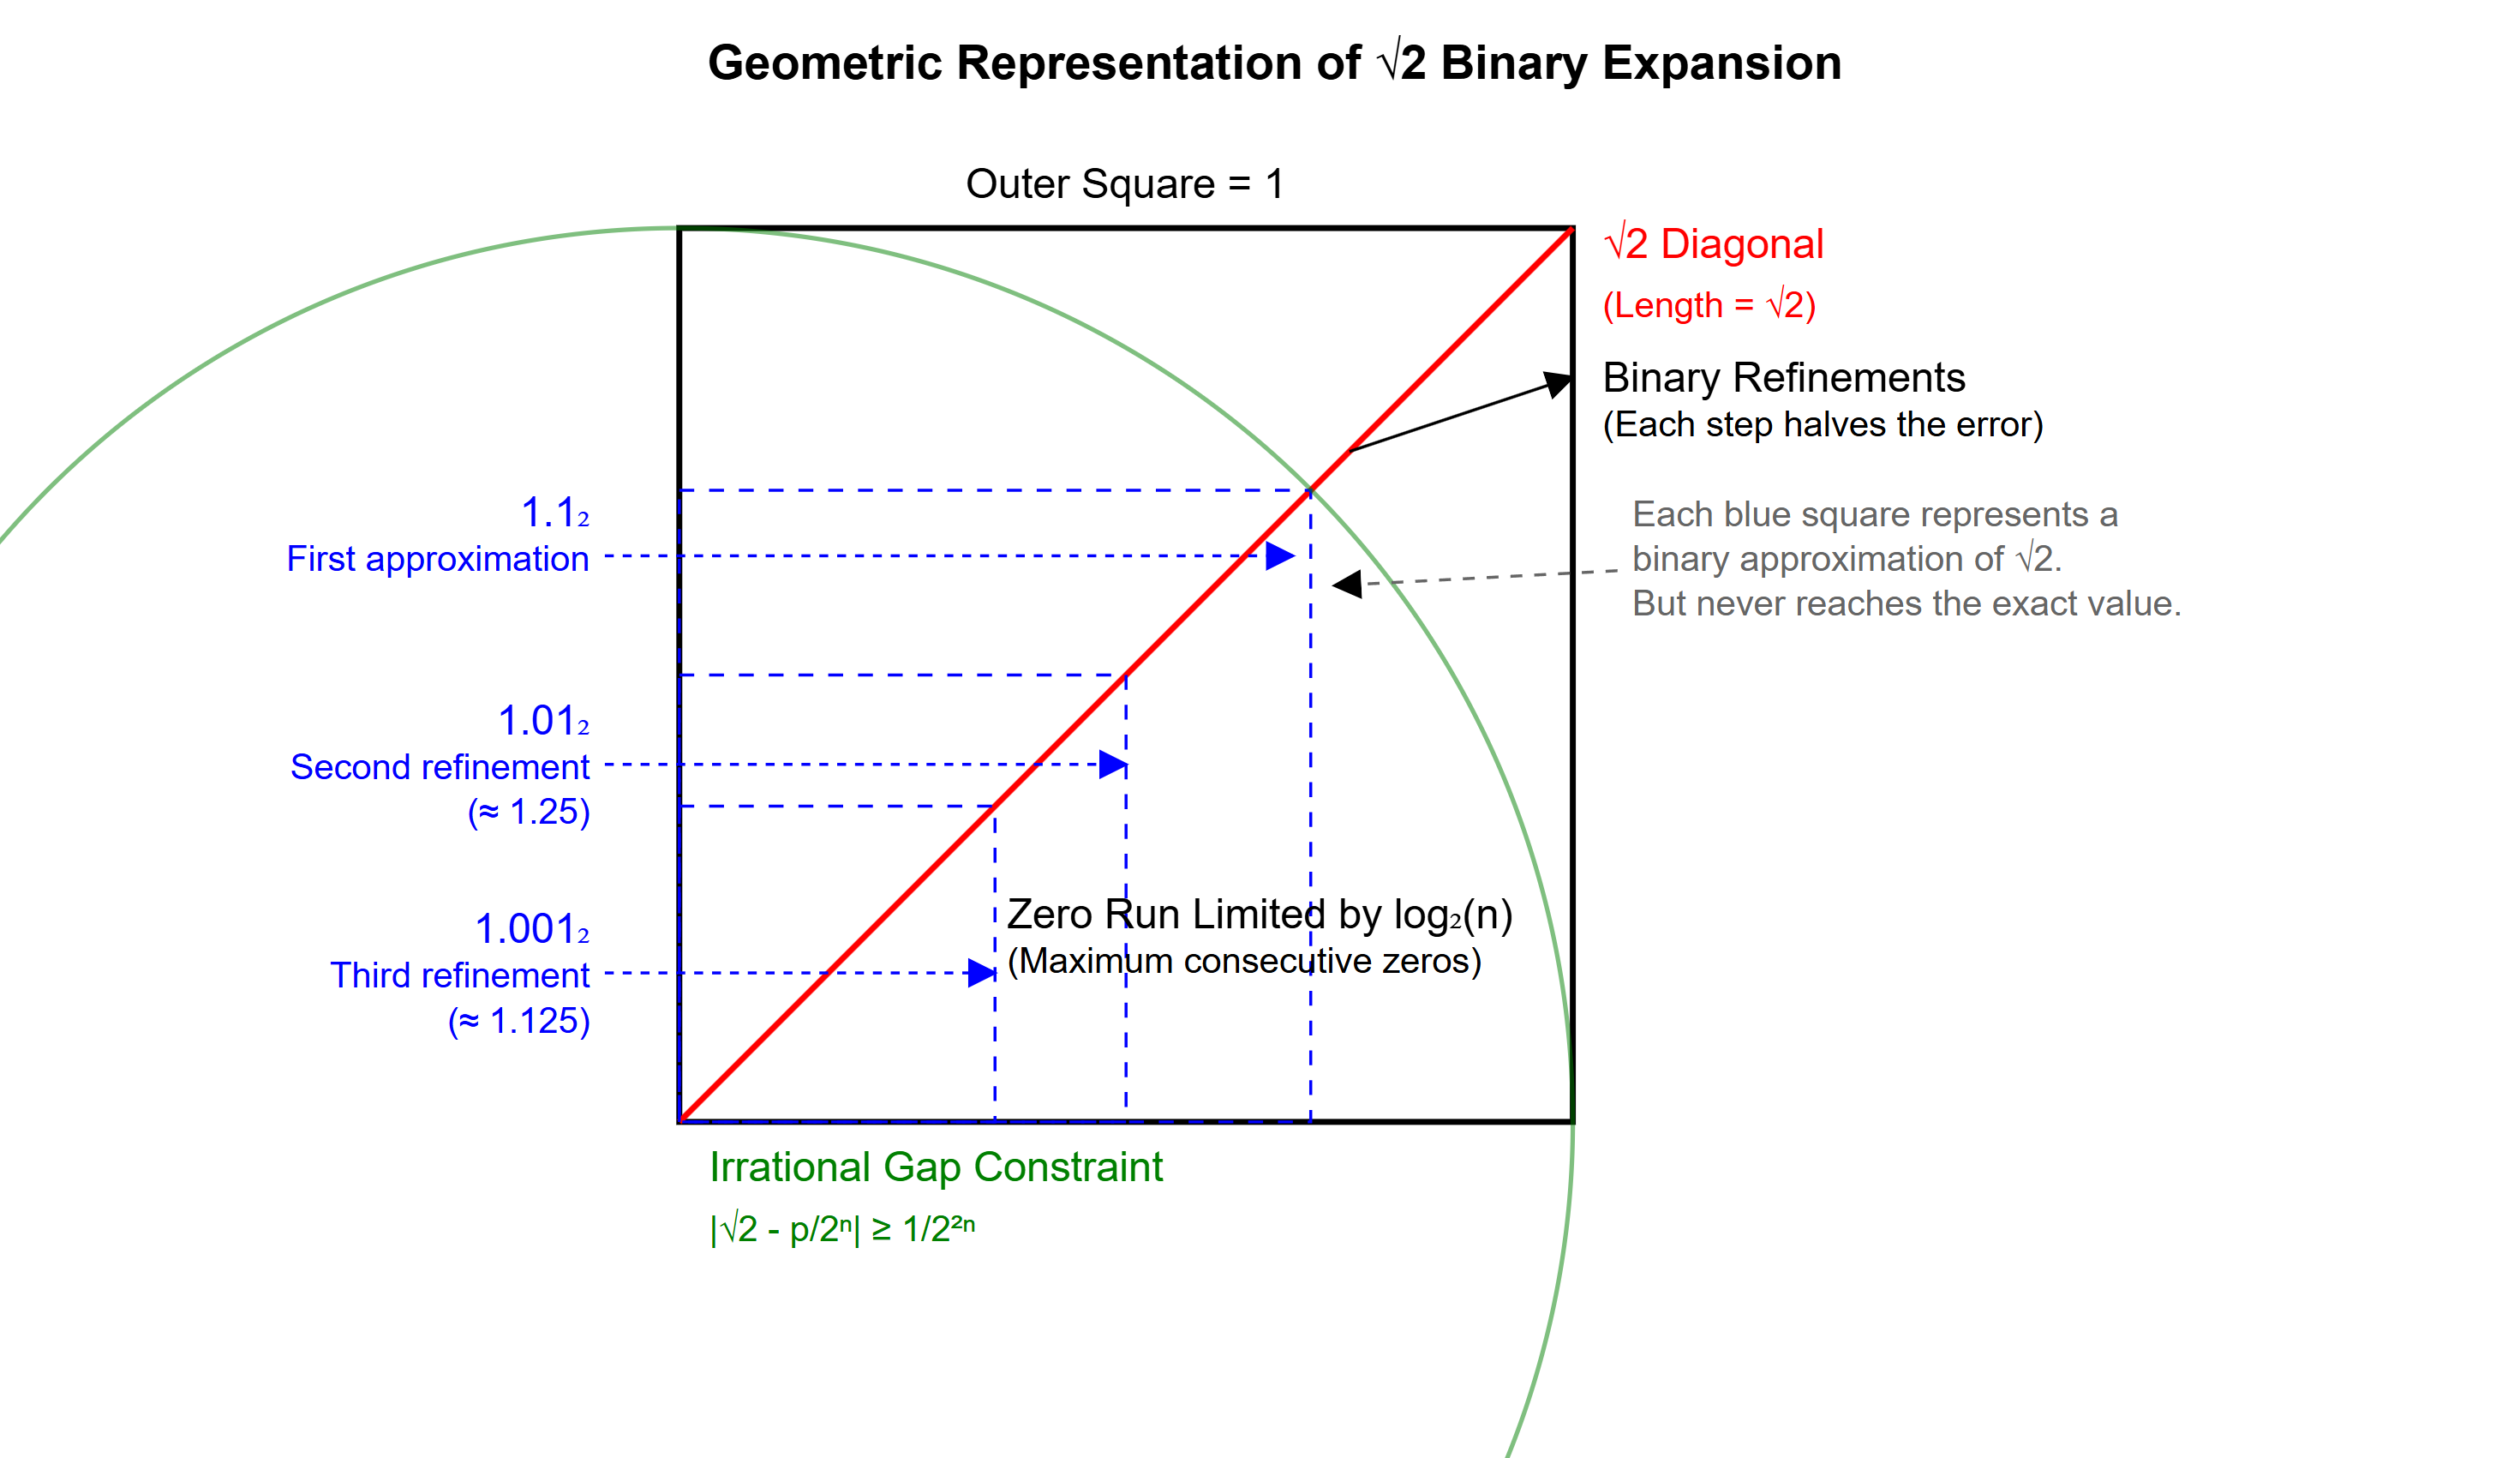
\includegraphics[width=0.8\textwidth]{geometric_diagram_illustrates.png} % Replace 'diagram.pdf' with your PDF file name
\end{center}

\subsection{Conclusion}
The geometric perspective provides intuitive understanding of why the binary expansion of $\sqrt{2}$ cannot have arbitrarily long runs of zeros. The fundamental relationship between the square and its diagonal, combined with the discrete nature of binary fractions, enforces this limitation.

